\chapter{Model Construction}
This chapter introduces a model based on Social Graph, which is the underlying structure to support Graph Search, the searchable encryption approaches and secure index for this model will be further discussed. In the last part of this chapter, a boolean query function will be presented on this model.

\section{Social Graph and Modelling}
As mentioned in \cite{curtiss2013unicorn}, Social graph is a directed graph consists of nodes which are describing the entities (users and user-generated contents like photos, pages) and edges as the relationships in social network. Social graph is a huge graph which contains many billions of nodes, however it is also a sparse graph, because most of the nodes only have no more than a thousand links between other nodes, while only a tiny fraction of nodes can attract tens of millions of links from others. As a result, in Unicorn \cite{curtiss2013unicorn}, the social graph can be represented by adjacent lists, and it stores as key-value pairs for query. 

In addition, there are various relationships in a social graph, the most common relationship is ``friends'', and a typical user may have up to a hundred friends. The interaction between nodes generates more relationships: For example, users can give a positive feedback to a restaurant by using ``likes'' on their page, it creates the ``likes'' relationship between user and page. In conclusion, the edges in social graph are labeled like a weighted graph, but a descriptor of relationship is used instead of a numeric weight. The relation label on edge can help to further reduce the size of adjacent lists. Moreover, the adjacent lists can be indexed not only by the node identifier but also the relationship type between its neighbours, such adjacent lists enable the content search in user's social network.

The generalised social graph model is defined on the basis of above facts. Formally, social graph is a edge-labeled and directed graph $G = (V, E)$, where $V = \{v_1, v_2, ..., v_n\}$ and $E = \{e_1, e_2, ..., e_m\}$, the total number of nodes is $n = |V|$, and the number of edges is $m = |E|$. There are several relationships $R$ associated with edges in social graph, all edges in $G$ can be represented as a triad $e = (u, v, r)$ which consists of its egress, ingress nodes ($u$ and $v$) plus a relationship $r\in R$ as its label. 
After introducing the notation of graph, the database based on it can be presented as follows: The social graph database $\mathbf{DB} = (ind_i, V_{{ind}_{i}})_{i=0}^{d}$ is an adjacent lists indexed by $ind = (u, r)$ which consists of egress nodes $u$ and a relationship $r$, the size of the database is proportional to the number of nodes $d \propto n$. 
A query takes an index $ind$ as input and returns a node list $V_{{ind}} \subseteq V$ subjects to the conditions $\{v\in V_{{ind}} | \exists e\in E \land e= (u, v, r)\}$.The complexity of such a query can be considered as a constant because $\mathbf{DB}$ is based on adjacent lists. The boolean queries on this database can take multiple indexes $ind_1, ind_2, ..., ind_t$ as input and get conjunctive result by $\mathbf{DB}(ind_1)\cap \mathbf{DB}(ind_)\cap ... \cap \mathbf{DB}(ind_t)$, the disjunctive queries can be done in the same way. 

\section{Searchable Encryption on Graph and its index}
The searchable encryption notion can be applied to the Social Graph model by introducing the concept upon the $\mathbf{DB}$. Let $\lambda$ be the security parameter, the searchable encryption scheme $\Pi$ consists of two algorithms:
\begin{itemize}
\setlength{\itemsep}{0pt}
\item $\mathbf{EDBSetup}(1^{\lambda}, \mathbf{DB})\rightarrow (mk, param, \mathbf{EDB})$: Run in client side, takes $1^{\lambda}$and $\mathbf{DB}$ as inputs and returns the system master key $mk$, public parameters $param$ and encrypted database $\mathbf{EDB}$. $mk$ is kept by client. $param$ is publicly known and $\mathbf{EDB}$ is stored in the server.
\item $\mathbf{EDBSearch}(mk, param, ind, \mathbf{EDB})\rightarrow (\mathbf{DB}(ind))$: $\mathbf{EDBSearch}$ runs between client and server as a protocol. Client?s inputs are $mk$, $param$, and query over $ind$, while server's inputs are $param$ and $\mathbf{EDB}$. At the end of the protocol, client outputs node lists matching query over $ind$, and server outputs nothing.
\end{itemize}

An overview of Search Encryption System on Graph is shown in Fig. \ref{fig:system}. The system involves two parties: the user and the server in untrusted cloud. During the $\mathbf{EDBSetup}$ phase, User can establish relationships with other users and upload these relationships into cloud server in an encrypted form. And in $\mathbf{EDBSearch}$ phase, user generates a search token related to the index $ind = (u, r)$ and send it to the cloud server, the server runs $\mathbf{EDBSearch}$ to retrieve requested results from encrypted Graph data without decrypt it and send it back to client. User can decrypt it on his/her local device.
\begin{figure}[h]
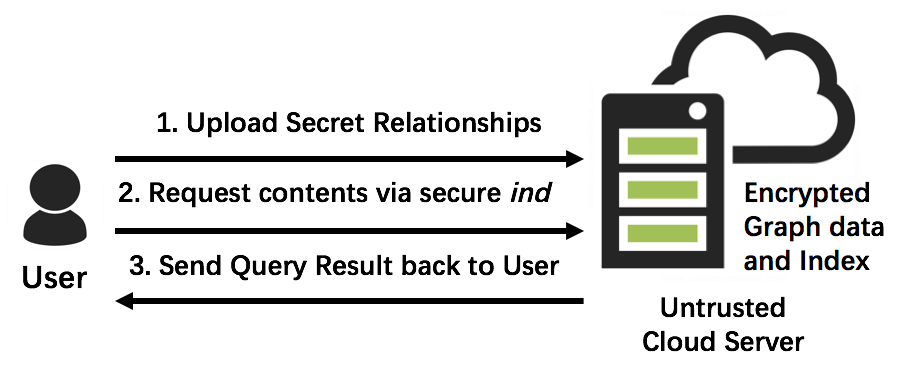
\includegraphics[width=\textwidth]{system.png}
\caption{System Architecture Overview}
\label{fig:system}
\end{figure}

Because of the index structure of $\mathbf{DB}$ is a typical inverted index. T-set can be used for efficient index on it. A T-set is an expanded inverted-index data structure \cite{cash2013highly} used for efficient SSE. It is a cryptographic data structure that associates a list of fixed-length data tuples to each keyword in a database. Later it enables the owner to issue corresponding tokens to retrieve these lists related to the queried keywords. A syntax, a correctness definition, a security model, and an instantiation of such a hash table is given in \cite{cash2013highly}. In the context of graph database, $ind$ can be used as the keyword of this database, and a T-set can be set to provide secure index for single keyword search in encrypted graph database.

\section{Boolean Queries in Graph Encryption}
Boolean queries are a fundamental functions for a database. In Graph database, boolean queries are used to get nodes with two or more relationships, and such queries are ubiquitous in our daily lives, for example, to get restaurants from friends, the query ``The restaurants visited by friends live in Melbourne'' is actually the composition of query ``Friends live in Melbourne'' and ``The restaurants visited by friends''. Furthermore, boolean queries also serve as the basis of many other rich type queries. Therefore, it is also necessary to support boolean queries in Graph Encryption because it is widely use and its importance to other queries.

A naive solution is to perform single keyword search on encrypted database multiple times, and let server or client to do intersections by theirselves. \cite{cash2013highly} pointed out that this solution is not efficient and has a significant leakage that leaks the sets of documents matching each keyword. There are some SSE constructions that only leaks the matching documents \cite{curtmola2011searchable} but it is not efficient in large database, because the conjunctive queries require to do $O(d)$ work on server side, where d is the number of documents or records in the database (many billions in social graph). 

To address the efficient and security issues, Cash et al. proposed `OXT' protocol, which also can be applied in graph encryption. The protocol is based on T-set and the concept of ``Oblivious tag''. 
In particular, the client sends the server a `search token' (called a $\mathbf{stag}$) related to the index $ind_1$ (called the `s-term' and denoted by $\mathbf{sterm}$), which allows the server to retrieve from the $\mathbf{TSet}$, the set $\mathbf{DB}(ind_1)$ of all nodes. In addition, the client sends `intersection tokens' (called $\mathbf{xtrap}$) related to the $n-1$ index \emph{pairs} $(index_1,index_i)$ consisting of the `s-term' paired with each of the remaining query index $ind_i$, $2\leq i \leq n$ (called `x-terms'). 
The intersection tokens allow the server to \emph{filter} the set $\mathbf{DB}(ind_1)$ to determine the $n-1$ subsets of nodes $\mathbf{DB}(ind_1) \cap \mathbf{DB}(ind_i)$ that contains the pairs $(ind_1, ind_i)$, returning only those nodes that contain all $\{ind_i\}_{1\leq i\leq n}$. 
The intersection subsets $\mathbf{DB}(ind_1) \cap \mathbf{DB}(ind_i)$ are efficiently computed by the server using the `$\mathbf{XSet}$' data structure; the `$\mathbf{XSet}$' is in essence a list of hashed pairs $h(ind, \mathbf{id_v})$, over all database node identities $\mathbf{id_v}$ and index $ind$ contained in $\mathbf{id_v}$, where $h$ is a certain (public) cryptographic hash function. 
To filter $\mathbf{DB}(ind_1) $ to compute $\mathbf{DB}(ind_1)  \cap  \mathbf{DB}(ind_i)$, the server runs through each node identifier $\mathbf{id_v}$ in $ \mathbf{DB}(ind_1)$ and checks, using the $\mathbf{xtrap}$ token for $(ind_1, ind_i)$ whether $h(ind_i, \mathbf{id_v})$ is in the $\mathbf{XSet}$. 
Therefore, the server computation time is dominated by $|\mathbf{DB}(ind_1)|(n-1)$ evaluations of $h$, which is proportional to just the number of nodes
containing the \emph{least frequent} `s-term' $ind_1$, even if other `xterm' indexes are much more common. 

The ideal searchable encryption only leaks Whole Result Pattern (WRP) in this result pattern (i.e. the number (and possibly also, identities) of documents matching all query keywords). However, in OXT protocol has leakages other than WRP in boolean query, because it has Keyword-Pair Result Pattern (KPRP): for an $n$ index conjunction query $ind_1 \wedge \cdots \wedge ind_n$, with $ind_1$ designated as the `s-term' index, the KPRP reveals to the server the set $\mathbf{DB}(ind_1) \cap \mathbf{DB}(ind_i)$ of documents containing every \emph{pair} of query keywords of the form $(ind_1, ind_i)$, $2\leq i\leq n$.

The new construction from this research named HXT eliminates KPRP leakage in state-of-art OXT protocol while leaves other query and result pattern leakage components in existing SSE protocols unchanged. Thus, in terms of security, our protocol offers strictly better guarantees than OXT protocol. Significantly, this improved security is obtained while preserving, within moderate constant factors, the practical high performance, in terms of server computation complexity, and storage, offered by OXT protocol.

To remove the KPRP leakage of OXT, a main idea of our protocol HXT is the use of HVE to implement a type of \emph{ciphertext policy} searchable encryption supporting subset membership predicates. Our ciphertext policy protocol is a kind of `dual' to the HVE-based \emph{key policy} searchable encryption protocol for subset membership predicates presented in \cite{boneh2007conjunctive}. In our HVE-based scheme, a dataset owner can encrypt a set $S \subseteq T=\{1,\ldots,n\}$, for some positive integer $n$, into a ciphertext $c_S$, which specifies a `policy'. Using a master secret key $msk$, the owner can generate a search token $tk_{S'}$ for any subset $S' = \{s'_1,\ldots,s'_\ell\}$ of $T$. Using the token $tk_{S'}$ for $S'$ and the ciphertext $c_S$ for $S$, anyone can efficiently check whether $S' \subseteq S$ or not, without leaking any partial information if $S' \not\subseteq S$, e.g. whether any particular element $s'_i$ of $S'$ is in $S$ or not (note that in the scheme of \cite{boneh2007conjunctive}, the set $S$ is used to generate the token, while the set $S'$ is encrypted in the ciphertext). 
Given this subset membership searchable encryption protocol, a natural idea to apply it to eliminate KPRP leakage in OXT would be to use it to \emph{encrypt the `$\mathbf{XSet}$'} during set up: we let $S \subseteq T$ denote the $\mathbf{XSet}$ list of hashed pairs $h(ind, \mathbf{id_v})$, over all node identifiers $\mathbf{id_v}$ and indexes $ind$ contained in $\mathbf{id_v}$, and we encrypt $S$ into a ciphertext $c_S$ stored on the server using our HVE-based subset searchable encryption scheme. In the search phase with query $ind_1 \wedge \cdots \wedge ind_n$, the client issues the server a HVE search token $tk_{S'}$ for $S' = \{h(ind_i, \mathbf{id_v})\}_{i=2}^n$, $\mathbf{id_v} \in \mathbf{DB}(ind_1)$. This allows the client to check whether $S'\subseteq S$, i.e., whether $\mathbf{id_v}$ contains all $n$ indexes $\{w_i\}_{1\leq i\leq n}$, without revealing the KPRP information on whether $\mathbf{id_v}$ contains any particular pair $(w_1,w_i)$.

There are two main issues with the above basic idea: the first one is the storage overhead. HXT introduces a small (but negligible) false positive probability $P_e$ to use the classical notion of a Bloom filter \cite{bloom1970space} reduce the storage size of $\mathbf{XSet}$ to $m \approx 2\log_2(1/P_e)N$, $m$ is the number of bits in Bloom Filter, and $N$ is number of items in the filter. Another issue is the performance of HVE, because most of the construction of HVE has exponentiation and pairings during instantiation, which are not efficient when $msk$ are built over billions possible attributes (it happened in Bloom Filter). we proposed a new symmetric HVE without pairings to address this issue.

\section{Future Works}
In this chapter, a general model for social graph and the searchable encryption notation for the proposed model are established. Based on the model, some existing definitions and tools from SSE can be adapted to support the secure index on graph encryption. By applying these definitions and tools, this research designed a secure and efficient boolean query protocol for graph encryption. So far, I have finished the modelling of Searchable Graph Encryption and fundamental queries on it, this research will focus on more complex search functions that support ``apply'' and ``extract'' queries, which are important components for Graph Search service, and the formal security defines and proof in future.


